\begin{refsection}
\chapter{Experimental Hardware}

MST is a well diagnosed device and my work has involved a large number of plasma diagnostics both directly and indirectly. In this chapter I give a summary of them, their general capabilities, their limitations, and the method of their incorporation into my work. Particular attention is paid to the Ion Doppler Spectrometer II (IDS-II) as it is the diagnostic I was most involved with in a hands-on fashion.

\section{The Madison Symmetric Torus}\label{sec:MST}
The Madison Symmetric Torus is a reversed field pinch device located in Madison, WI. It was constructed in the 1980s, achieving first plasma in 1988.
\begin{figure}[!htb]
	\centering
	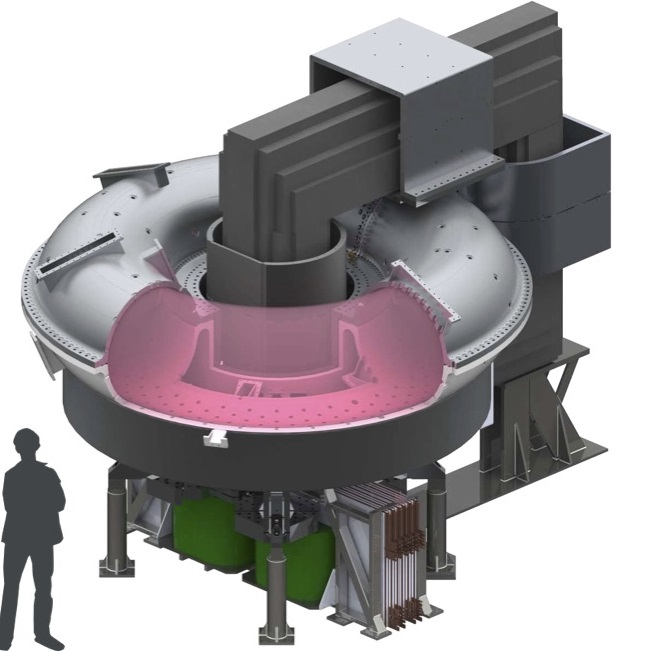
\includegraphics{./2_Experimental_hardware/MST_model_diagram}
	\label{fig:MST_diagram}
	\caption[Diagram of MST]{Diagram of MST. Note the close fitting shell, as well as the holes on the bottom of the vessel that leads to the pumping manifold. It's location will become relevant in section \ref{sec:neutral_dynamics}.}
\end{figure}

I work here!


\begin{figure}[!htb]
	\centering
	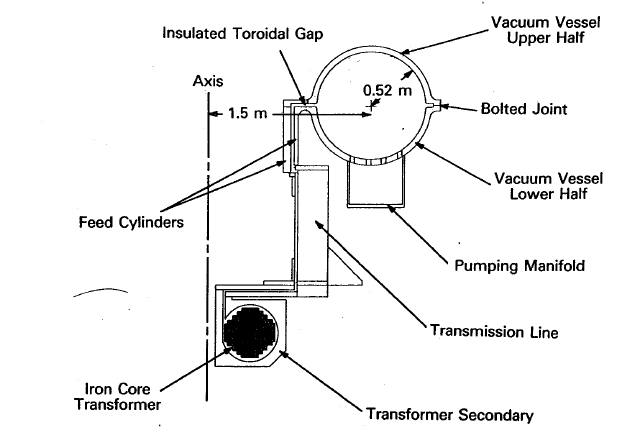
\includegraphics{./2_Experimental_hardware/MST_tor_section.PNG}
	\label{fig:MST_tor_section}
	\caption[Toridal section of MST]{Toroidal section diagram of MST. Note again pumping manifold's location; as well as the transmission line coupling the secondary transformer to the close fitting shell itself. This is what allows the inductive current drive behind PPCD operations. The entire shell is used as a 'TF coil'. (Reproduced from R. Dexter et al. Ref\cite{Dexter100}}
\end{figure}


\section{Magnetic coils, equilibrium reconstruction and MSTfit}
I trust Jay, and didn't look that carefully at any of it\cite{mstfit}.

\section{Far Infrared Interferometer and Polarimeter}
Gets me $n_e$ and $B$.

\section{The $D_{\alpha}$ array}
Gets me neutral information.

\section{The Thompson Scattering Thing}
It's not an interferometer and I don't think it's a spectrometer. So it's just a thing right now.



\section{The Ion Doppler Spectrometer II and Charge Exchange Spectrometry}
Gets me $T_{impurities}$

\printbibliography
\end{refsection}